\section{Technical Approach}
%=====================================================================

\subsection{Architecture and Deployment}

The platform is a layered client-server system. A mobile-first, component-based PWA built with React, TypeScript, and Vite serves Users, Staff, and Administrators from one codebase on phones and desktops, so no separate iOS and Android apps are needed. A Laravel API [10] (PHP 8.3 or higher) holds the business rules: authorization, Check In, sessions, imports, and role checks. PostgreSQL is the source of truth for users, academic terms, authorizations, athlete rosters, sign-in sessions, facility sessions, roles, waiver acceptances, and the audit log. Photographs sit on a private volume that only the API can read. Backend time decides the 60-minute expiration. WooCommerce remains the paid-membership source, read through an Export Orders file that an Administrator uploads.

The proposal named Supabase and Vercel. The team replaced them with a stack that CTI can host in December: the same PWA, Laravel, PostgreSQL, and nginx, all started by one \texttt{docker-compose} file that runs on each member's computer and on a CTI virtual machine (VM). No student data sits in an outside service, and what the team tests is what runs in production. Laravel replaces Row Level Security and Edge Functions with policies, middleware, and database constraints. Occupancy screens poll the API every 20 to 30 seconds instead of using real-time channels, because occupancy changes only at a Check In or an expiration. Live updates may be added later if CTI allows them and time remains. \pending{professor approval of the stack change}

\subsection{System Architecture}

\textbf{Components.} Everything runs as containers on one host, and only the proxy publishes a port.
\begin{itemize}
  \item \textbf{Proxy (nginx):} ends HTTPS and applies two rules: \texttt{/api} goes to Laravel, everything else goes to the PWA files. The app and the API share one origin, so cookie sign-in needs no cross-site settings.
  \item \textbf{PWA:} static files built by Vite. The service worker never caches API responses, so stale data is not shown as current.
  \item \textbf{App (Laravel on PHP-FPM):} the API under \texttt{/api}, Laravel policies for roles, and the WooCommerce import.
  \item \textbf{Scheduler:} the same image as the app, running scheduled tasks such as marking old sessions expired and discarding old-term photographs.
  \item \textbf{Database (PostgreSQL) and photo volume:} the database enforces one active session per User and one claim per Authorization Number or roster record.
\end{itemize}
Outside the host, the browser Geolocation API supplies position and accuracy at Check In only. Outgoing mail carries invitations, athlete links, and password resets: a fake mail server in development and the CTI mail gateway in production. A compromised-password check sends only the first five characters of a password hash and no student data.

\textbf{Check In request path.} Figure~\ref{fig:architecture} shows the components; the Check In path through them has seven steps.
\begin{enumerate}
  \item The User taps Check In. The PWA sends an eligibility query over HTTPS with the session cookie, and the proxy forwards it to Laravel.
  \item Middleware confirms the cookie is the User's current sign-in session. The API then reads authorizations, the academic term, the schedule, and any active facility session.
  \item If a session is active, the API returns it with the Gym ID and asks for no location. If a check fails, it returns a fixed cause code, and the app writes the message in the account's language.
  \item If the User is eligible, the API asks for location. The PWA reads it from the browser and sends the position and accuracy to \texttt{POST /api/check-in}.
  \item The API repeats every check, then tests accuracy and the gym boundary.
  \item The API inserts the facility session in one transaction. A PostgreSQL exclusion constraint on the time range rejects an overlapping session from a simultaneous request, and the API returns the existing session instead.
  \item The PWA shows the Gym ID. Coordinates are never stored, only the result of the check.
\end{enumerate}

\textbf{Deployment.} In development, each member runs the full stack with Docker Desktop. Phones reach it through an HTTPS tunnel because the Geolocation API requires HTTPS. Production is a CTI VM with a UPRM subdomain and HTTPS, filed by the project owner. The December demo runs in a separate environment with its own database and the classroom boundary. The production app refuses to start if the configured boundary is more than 50 meters from the gym, so the classroom boundary cannot reach production by a missing setting. Images use pinned versions, and server credentials stay in protected configuration outside the repository. \pending{CTI answers: VM operating system, HTTPS certificate, mail gateway authorization, and backup method}

\subsection{Identity, Authorization, and Session Model}

\begin{itemize}
  \item \textbf{Account and role:} the persistent person, who survives across semesters. Each person has an individual account with one role: User, Staff, or Administrator.
  \item \textbf{Semester authorization:} whether a User currently has access. A User may have several authorization records over time and may move between paid-member and athlete authorization without a new account.
  \item \textbf{Sign-in session:} the device currently signed in.
  \item \textbf{Facility session:} the 60-minute period created by a successful Check In.
\end{itemize}

\textbf{Roles and invitations.} Staff and Administrator accounts are individual. An Administrator invites each person by email, and the invited person sets a password. The shared gym account, the Administrator PIN, and the paper recovery code from the earlier design are removed. An install command creates the first Administrator. Staff verify Gym IDs, make Staff-assisted Check Ins and session corrections, and read the current roster. Administrators also manage terms, rosters, imports, schedules, notices, facility information, accounts, and the audit log. Laravel policies check each action by role. The audit log names the person who acted, with time, IP address, device, and the values before and after.

\textbf{Sessions.} Sign-in uses Laravel Sanctum cookie sessions with Fortify for sign-in and password reset. Both are proposed in the design documents and not yet in the code. After 10 failed attempts, counted per account and per IP address, that account or address waits, and the wait grows with each lockout. Only one device may stay signed in to a User account: a successful sign-in on another device ends the previous session, which can no longer perform protected actions. There is no inactivity timeout, because a timeout could sign a User out between Check In and the front desk. The one-device rule applies to Users only.

\textbf{Passwords.} A password needs at least 10 characters, and the system accepts at least 64. There are no composition rules. When a password is set or changed, Laravel's \texttt{uncompromised} rule checks it against known breached passwords using only a five-character hash prefix. NIST SP 800-63B-4 asks for at least 15 characters when a password is the only factor [8]. The team chose 10 because people type passwords on a phone, and it records this as a deviation. A reset request gets the same answer whether or not the email has an account.

\textbf{Facility sessions.} Academic terms are separate from individual purchases. A fall membership ends at the end of the configured fall semester even if bought later. A User may have only one active facility session. A second Check In during an active session returns the existing session, and a later valid Check In after expiration creates a new one. The backend evaluates timing, so expiration does not depend on a user action or on the interface staying open.

\subsection{WooCommerce Membership Integration}

WooCommerce remains the authoritative source for paid-membership purchases. The team has authorized access to WooCommerce Orders and Export Orders, and the export includes the Authorization Number that paid registration needs. An Administrator uploads an Export Orders file; there is no API link in the first version. A file with an unexpected format imports nothing. \pending{Export Orders columns, awaiting an authorized sample file}

Only the fields needed for authorization are copied into PostgreSQL: name, email, student number when present, membership details, Authorization Number, order reference, status, payment date, term, and last synchronization time. Billing and address data are not copied. An order belongs to the term that contains its payment date, and an order dated outside every term is rejected and listed in the import result. The Authorization Number is unique per term, so one membership cannot be claimed by two accounts.

The gym does not refund memberships, so the integration handles no refunds or cancellations: a membership only expires at the end of its term. An Administrator can re-import a corrected file, and processing the same order twice updates or confirms the same record instead of creating a duplicate. Any import can also be undone. Undo deletes the membership records that import brought, the authorizations that depend on them, and their term photographs. Accounts stay, and people claim again with a new photo. Each import result is saved with every created, updated, and rejected row, so an Administrator can reopen it later. Registration does not depend on scanning WooCommerce, and a later API or webhook link would update the same local records.

\subsection{User Interface Design}

The screen map lists every screen of the PWA, with its roles, purpose, key states (loading, empty, error, no connection), and the requirements it serves. It has 45 screens: 12 for people who are not signed in, 9 for Users, 6 shared by all roles (occupancy card, schedules, notices, facility information, analytics, language), 5 for Staff, and 13 for Administrators. Seven navigation maps show how a person moves between screens: public, User with an active authorization, User without one, Staff, Administrator, the shared app frame, and the standard data states. Users get a phone-first layout, because about 150 people a day use it, and Check In is the first screen after sign-in so it loads in under 3 seconds. Staff and Administrator screens are desktop-first for the front desk computer, which the gym still has to confirm, and they share the PWA codebase. Without a connection, no session is created and the app shows a banner that the data is not current. Accessibility notes in the screen map cover dialogs, the moving Gym ID clock, status messages, and tap-target sizes. The screen map was written before the account change, so the PIN and recovery-code screens will give way to invitation and sign-in screens. \pending{screen map update for individual accounts}

The wireframe guide splits the work into six issues of 45 screens: registration (9, \#40), Check In and Gym ID (3, \#41), sign-in and account (13, \#42), Staff (5, \#43), content and analytics (7, \#44), and administration (8, \#45). \pending{wireframe figures from \#40 to \#45}

\subsection{System Diagrams}

The following five diagrams show the platform architecture, account creation, authorization lifecycle, Check In sequence, and conceptual data model, as drawn for the proposal.

% --------------------------- FIGURE 1 ------------------------------
\begin{figure}[!htbp]
\centering
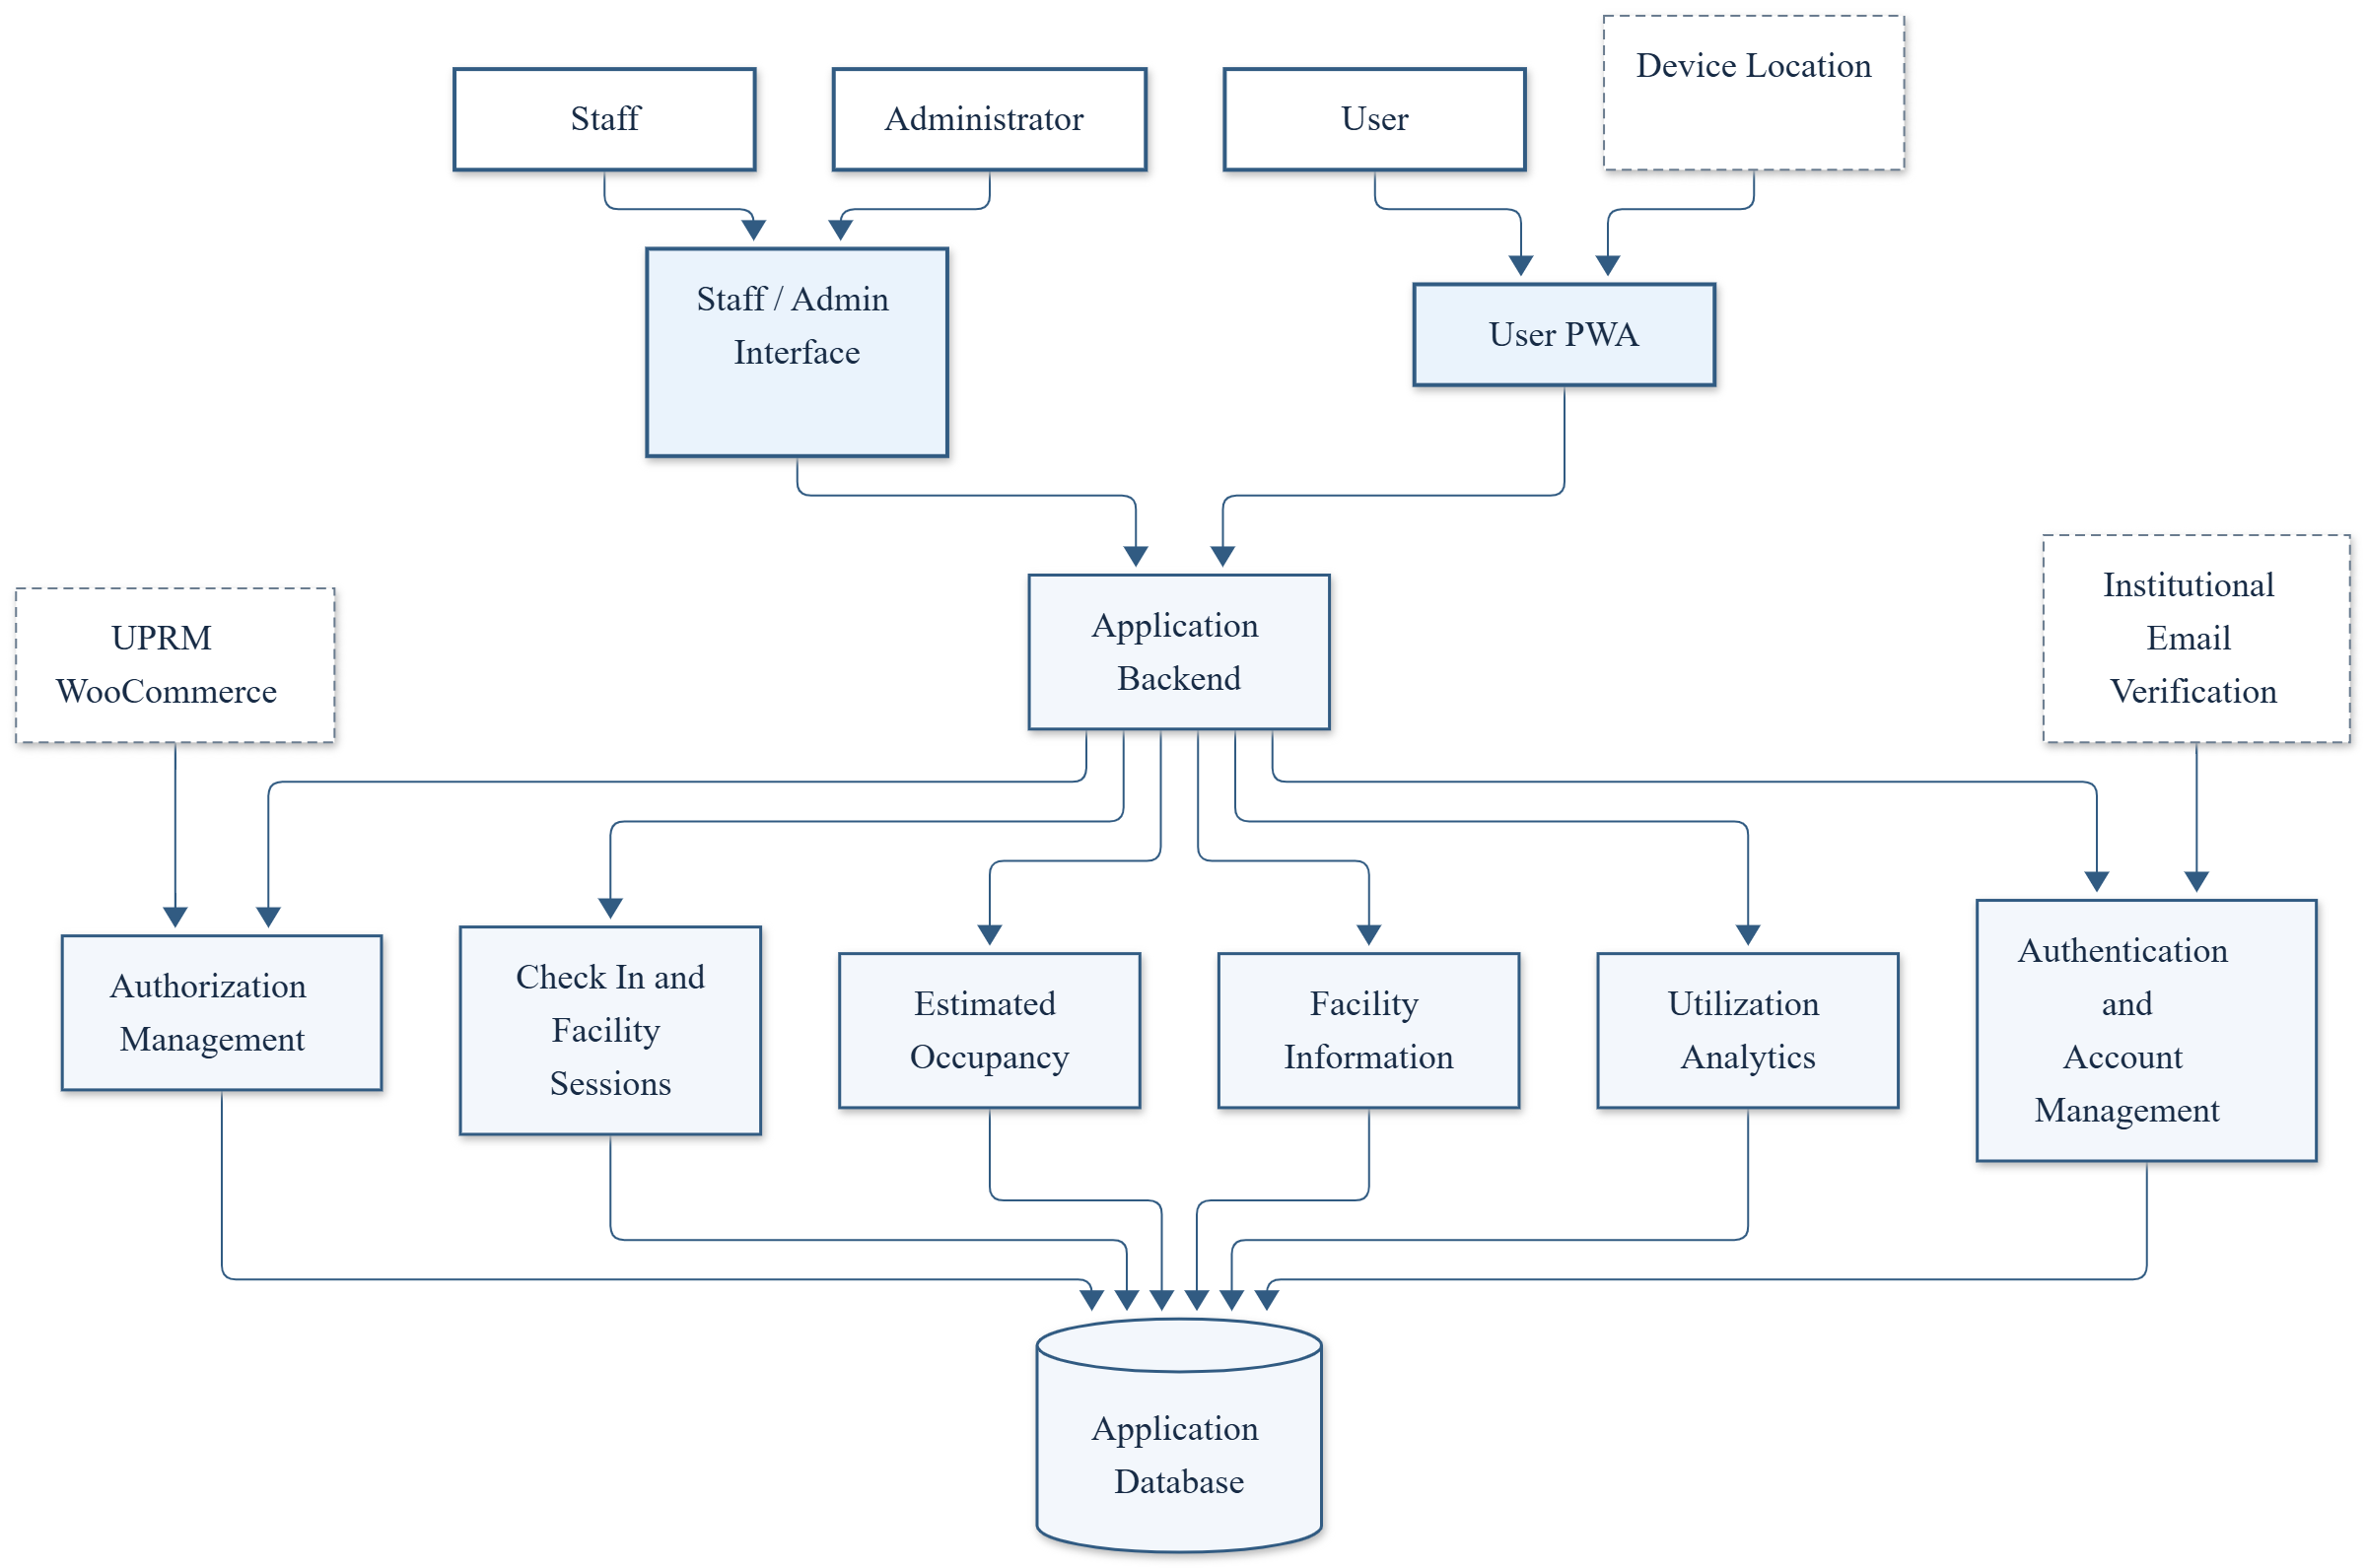
\includegraphics[width=0.9\textwidth,height=0.45\textheight,keepaspectratio]{diagrams/01_architecture.png}
\caption{High-Level System Architecture}
\label{fig:architecture}
\par\vspace{0.35em}\noindent\small\RaggedRight
Figure 1 shows how the User PWA and Staff/Administrator interface connect to the backend, its services, and the application database. WooCommerce, institutional email verification, and device location supply information to the relevant workflows. The figure still shows the proposal's stack. \pending{replace Figure 1 with the container diagram from the architecture document}
\end{figure}

% --------------------------- FIGURE 2 ------------------------------
\begin{figure}[!htbp]
\centering
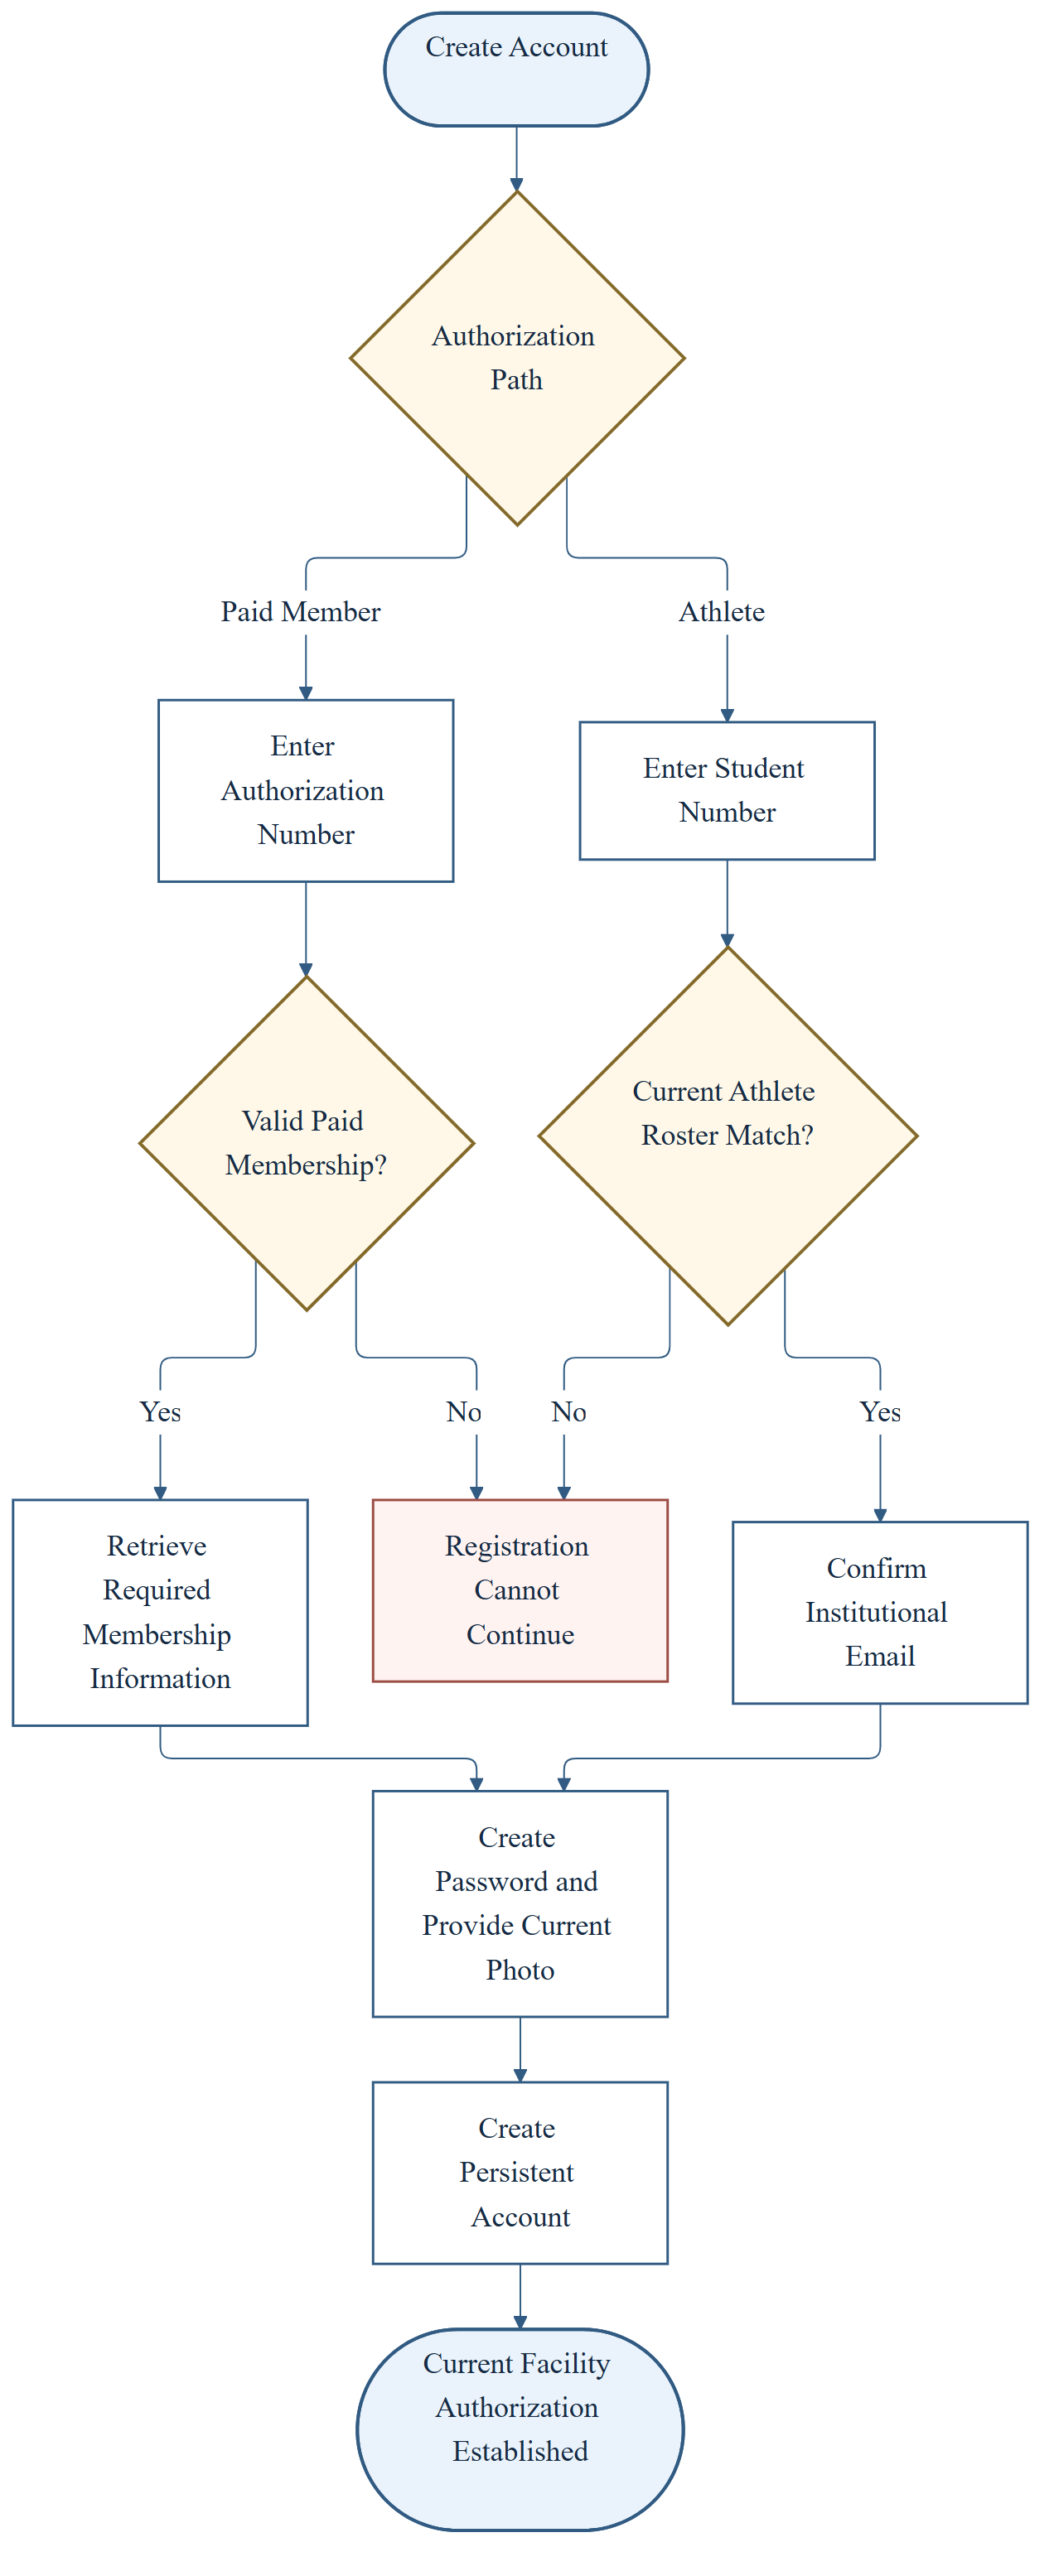
\includegraphics[width=0.98\textwidth,height=0.6\textheight,keepaspectratio]{diagrams/02_account_creation.png}
\caption{Paid-Member and Athlete Account Creation}
\label{fig:accountcreation}
\par\vspace{0.35em}\noindent\small\RaggedRight
Figure 2 separates paid-member validation by Authorization Number from athlete validation against the current roster. Both paths then create one persistent account with a password and current photo. \pending{refresh Figure 2: the Authorization Number lookup limits, the emailed link that creates an athlete account, the photo saved together with the account, and the Staff one-time code}
\end{figure}

% --------------------------- FIGURE 3 ------------------------------
\begin{figure}[!htbp]
\centering
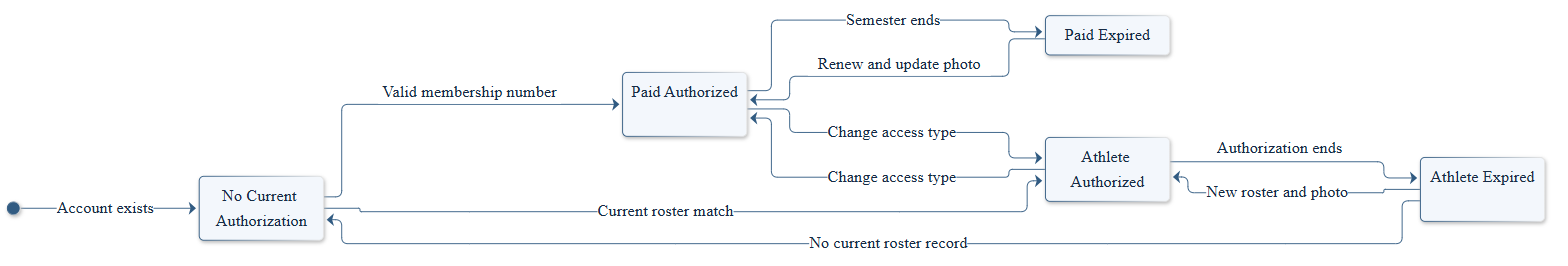
\includegraphics[width=0.98\textwidth,height=0.3\textheight,keepaspectratio]{diagrams/03_authorization_lifecycle.png}
\caption{Post-Registration Account and Authorization Lifecycle}
\label{fig:lifecycle}
\par\vspace{0.35em}\noindent\small\RaggedRight
Figure 3 begins after a persistent account has been established. Authorization may expire, be renewed, or change between paid-member and athlete access while the same User account remains intact. \pending{refresh Figure 3: renewal inside the same account with a new Authorization Number, the ``I am an athlete'' link, the new-term photo, manual grant and revoke, release of a mistaken claim, and import undo}
\end{figure}

% --------------------------- FIGURE 4 ------------------------------
\begin{figure}[!htbp]
\centering
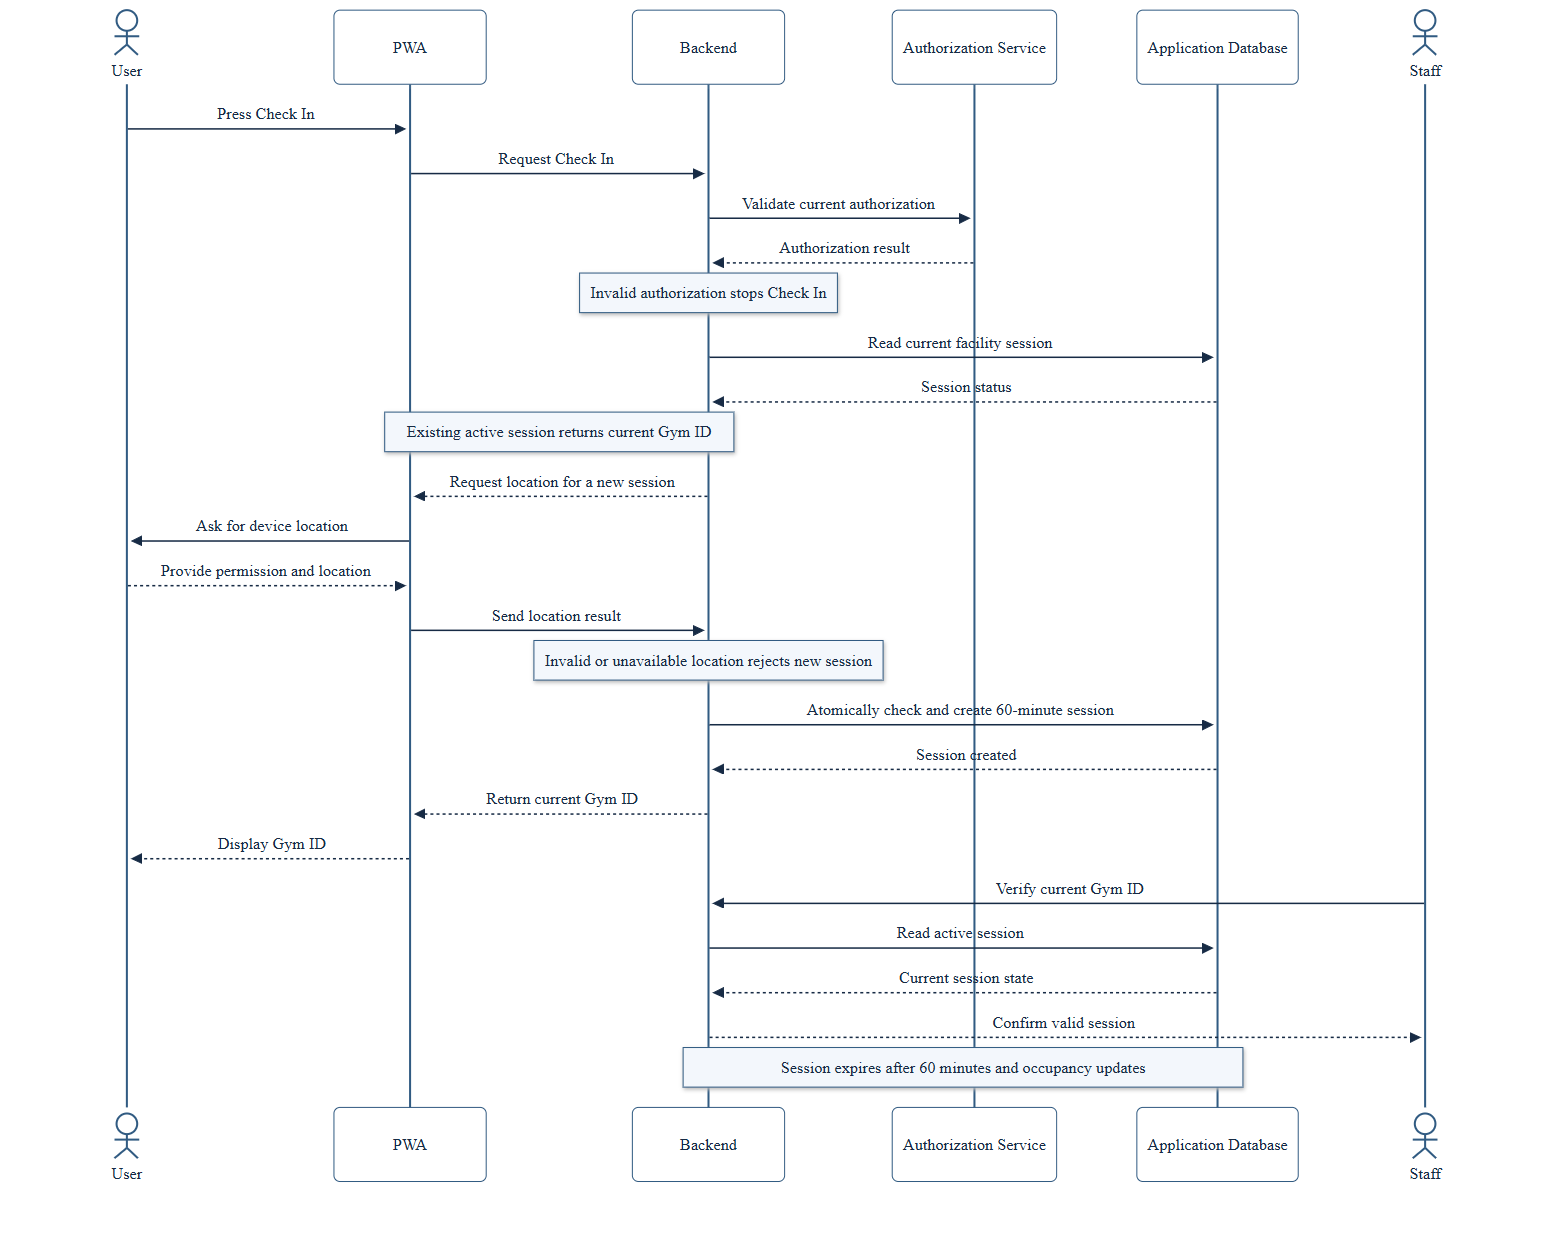
\includegraphics[width=0.98\textwidth,height=0.5\textheight,keepaspectratio]{diagrams/04_checkin_session.png}
\caption{Check-In and Facility Session Sequence}
\label{fig:checkin}
\par\vspace{0.35em}\noindent\small\RaggedRight
Figure 4 shows how authorization, location, active-session control, Gym ID, and Staff verification interact during Check In. The active-session check and session creation are one protected backend operation, so simultaneous requests cannot create overlapping sessions. Location is requested only when a new session is needed. \pending{refresh Figure 4: remove the separate Authorization Service (checks run inside the Laravel app), show the two-step flow with an eligibility query before the Check In request, the cause codes, and the database exclusion constraint}
\end{figure}

% --------------------------- FIGURE 5 ------------------------------
\begin{figure}[!htbp]
\centering
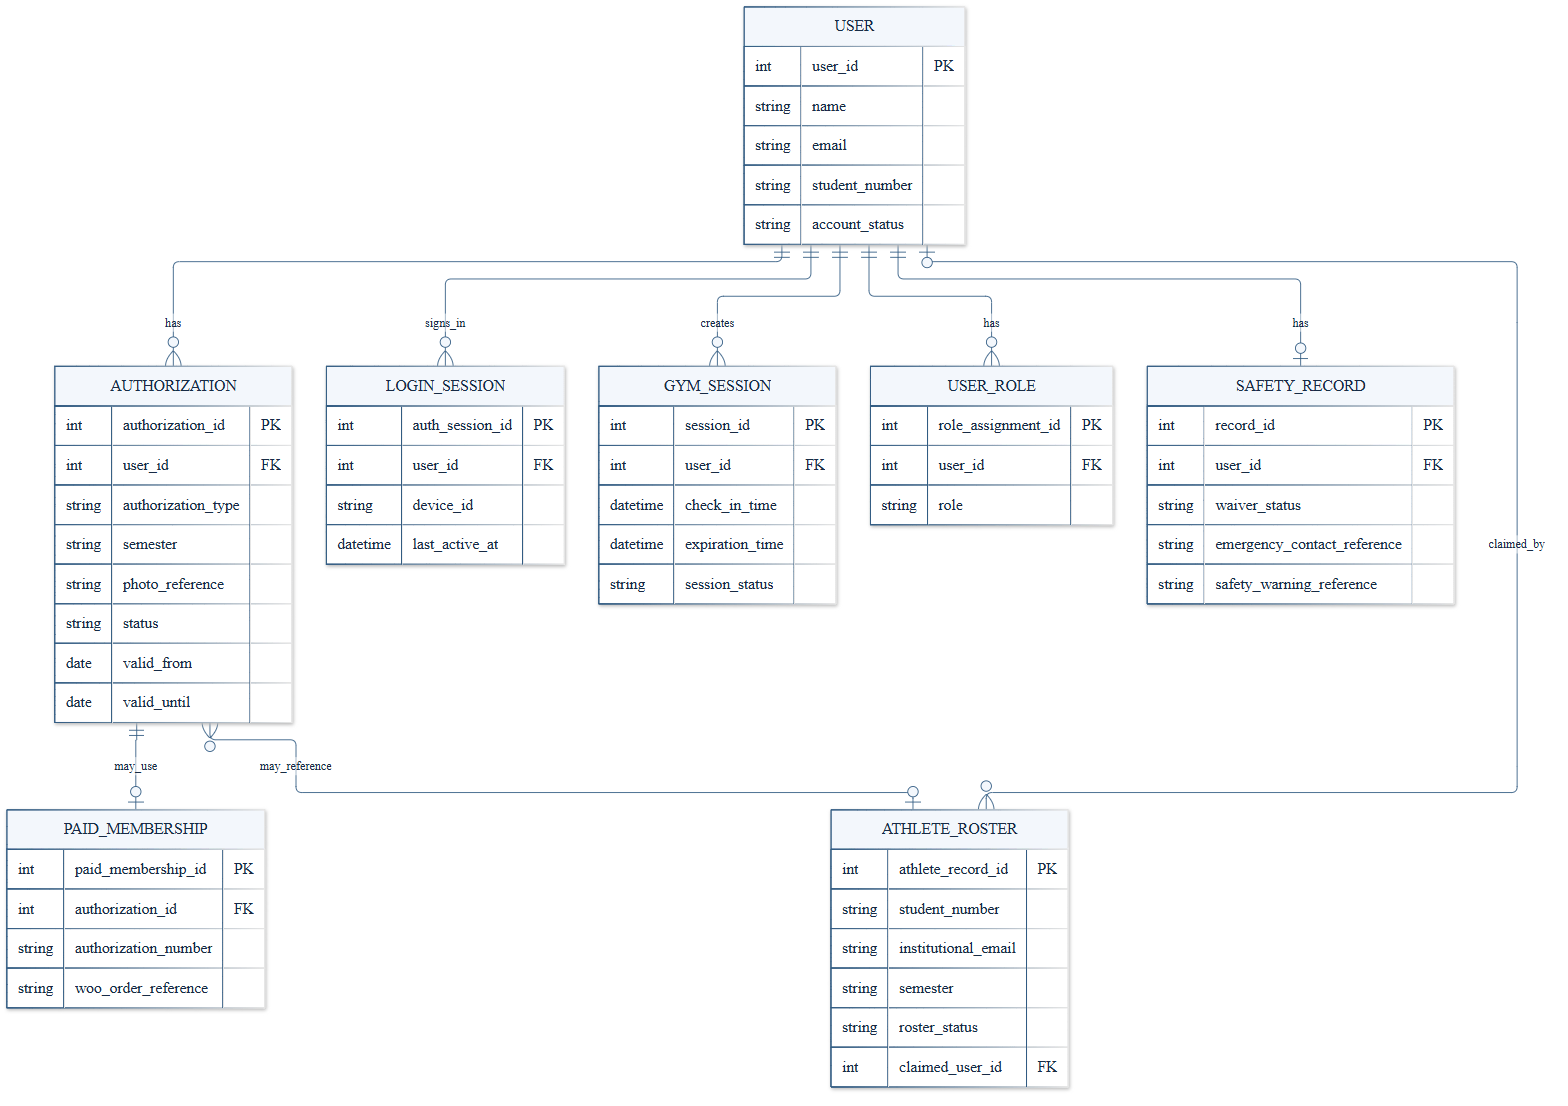
\includegraphics[width=0.98\textwidth,height=0.45\textheight,keepaspectratio]{diagrams/05_data_model.png}
\caption{Conceptual Data Model}
\label{fig:datamodel}
\par\vspace{0.35em}\noindent\small\RaggedRight
Figure 5 separates identity, authorization, sign-in state, facility sessions, roles, and protected membership information. The model keeps semester-specific photographs with Authorization rather than treating the photograph as a permanent User attribute. \pending{refresh Figure 5: add academic terms, imports, imported memberships, roster records, email links, and audit log entries; rename login session to sign-in session; reduce safety records to the waiver acceptance with an emergency contact}
\end{figure}

\subsection{Related Works}

\textbf{Progressive Web Applications.} Królikowski and Miłosz studied factors that affect PWA performance on mobile devices, including resource minimization, lazy loading, and distributed content delivery. The team uses their findings as performance guidance for the PWA [3].

\textbf{Indoor smartphone location.} NIST evaluated smartphone location technologies across five large buildings and found measurable differences in indoor localization performance between Android and iPhone. This supports treating device location as supporting evidence for Check In rather than exact proof of presence, and supports setting the final location boundary and accepted accuracy through tests at the actual Weight Gym [4].

\textbf{Role-Based Access Control.} The NIST RBAC model describes authorization in terms of users, roles, and permissions rather than direct access to every resource. It informs the separation of User, Staff, and Administrator privileges and supports keeping Developer/Maintainer access outside normal gym operational roles [5].

These works shape three engineering decisions: PWA performance, the treatment of indoor device location, and the access-control structure.

\subsection{Engineering Constraints and Verification}

\begin{center}
\small
\begin{longtable}{L{3.1cm} L{5.1cm} L{5.2cm}}
\toprule
\textbf{Constraint and reason} & \textbf{Engineering response} & \textbf{Pass condition / timing} \\
\midrule
\endfirsthead
\toprule
\textbf{Constraint and reason} & \textbf{Engineering response} & \textbf{Pass condition / timing} \\
\midrule
\endhead
\bottomrule
\endlastfoot
\textbf{WooCommerce source.} Membership data remains in an external system. & Keep WooCommerce authoritative, copy only needed fields, and load it from an uploaded Export Orders file so upstream changes do not redesign accounts. & Re-importing a corrected file produces no duplicate, and undo removes what the import brought (Phase 4). \\
\addlinespace
\textbf{Indoor location [4].} Phone accuracy varies by device and indoors. & Require a reading; compare gym boundary and reported accuracy; set the threshold through on-site tests. & Inside, outside, denied-permission, and low-accuracy cases pass on real phones at the gym (Phase 3). \\
\addlinespace
\textbf{Connectivity and polling.} Sign-in, authorization, sessions, one-device enforcement, and Gym ID verification need the backend, and occupancy refreshes by polling every 20 to 30 seconds. & Require connectivity; disable offline Check In to avoid inconsistent access and occupancy; never cache API responses in the service worker. & Offline Sign In and Check In create no session; every screen shows the same occupancy value after its next poll (Phases 3 to 4). \\
\addlinespace
\textbf{Concurrency.} Simultaneous requests can duplicate sessions or claims. & Enforce database uniqueness and exclusion constraints and atomic Check In, not frontend-only checks. & Concurrent requests and repeated Authorization Number or athlete-record claims yield one session or claim; a load test above the expected peak keeps occupancy correct (Phases 3 to 6). \pending{expected peak number from the gym} \\
\addlinespace
\textbf{Browser/device variation.} PWA and geolocation behavior vary. & Test real phones on iPhone/Safari and Android/Chrome; test Windows/Chrome and Edge, with secondary macOS/Firefox checks. & Core flows pass the defined device/browser matrix (Phases 3 to 6). \\
\addlinespace
\textbf{Accessibility.} Users, Staff, and Administrators may use a keyboard, a screen reader, zoom, or a small screen. WCAG 2.2 level AA is required (REQ-NF-13, REQ-NF-14, REQ-NF-36) [6]. & Show states with text or an icon, not color alone; change the page language with the texts; keep tap targets at least 24 by 24 pixels. Verify with axe-core run through Playwright in CI, oxlint jsx-a11y rules, and a manual checklist: keyboard only, NVDA, VoiceOver, 200\% zoom, and a 320 pixel width. & No axe violations on any screen in CI, and the manual checklist passes on the main flows (issue \#82). \\
\addlinespace
\textbf{Sensitive data.} Photos, waivers, emergency contacts, and the audit log need protection. & Restrict by role with Laravel policies, use a private photo volume and minimal collection, and define retention; Staff see only Check In essentials. & Role-permission tests confirm least-needed record access (Phase 5). \\
\addlinespace
\textbf{Mail dependency.} Invitations, athlete links, and password resets need outgoing mail. & Send mail during the request. Use a fake mail server in development and the CTI mail gateway in production, with an external provider only if CTI declines and approves it. & Each link flow works end to end against the fake mail server in tests. \pending{CTI authorization of the VM on its mail gateway} \\
\addlinespace
\textbf{CTI VM.} CTI creates the VM and the domain, but does not manage or maintain the server or the application. & Run the same \texttt{docker-compose} file as in development, with pinned images, and agree a backup and restore procedure with the project owner. & The full stack starts from \texttt{docker-compose} on the VM, and a restore from backup works before the release (Phase 6). \pending{backup method and VM operating system from CTI} \\
\end{longtable}
\end{center}

\subsection{Engineering Standards}

Each standard below applies to a specific technology or risk of the platform.

\begin{center}
\small
\begin{longtable}{L{3.6cm} L{4.4cm} L{5.6cm}}
\toprule
\textbf{Standard} & \textbf{Application to the Project} & \textbf{Justification} \\
\midrule
\endfirsthead
\toprule
\textbf{Standard} & \textbf{Application to the Project} & \textbf{Justification} \\
\midrule
\endhead
\bottomrule
\endlastfoot

WCAG 2.2, relevant Level AA criteria [6]
&
User, Staff, and Administrator web interfaces
&
Targets accessible forms, navigation, touch interactions, and status information. Key states such as the live Gym ID use text or icons in addition to color. Checked by axe-core in CI, lint rules, and a manual checklist. \\
\addlinespace
\midrule
\addlinespace

W3C Geolocation specification [7]
&
Location-based Check In
&
Uses browser-provided geolocation through the standard API. Permission state and reported accuracy are handled in the Check In flow. \\
\addlinespace
\midrule
\addlinespace

NIST SP 800-63B-4, Digital Identity Guidelines: Authentication [8]
&
Passwords, password reset, and sign-in sessions for all accounts
&
Accepts at least 64 characters, sets no composition rules, rejects known breached passwords, limits failed attempts, and answers a reset request the same way for every email. The 10-character minimum deviates from the 15 the standard asks for passwords used alone, because people type on phones. \\
\addlinespace
\midrule
\addlinespace

OWASP ASVS 5.0.0 [9]
&
Authentication, session, and access-control design
&
Consulted for the controls above: hashed passwords, cookie sessions on one origin, per-account and per-IP attempt limits, one device per User, role checks on the server, and an audit log that names the person. \pending{control-by-control mapping and target ASVS level} \\
\addlinespace
\midrule
\addlinespace

NIST RBAC model [5]
&
User, Staff, and Administrator roles
&
Each action is allowed by role through Laravel policies rather than by direct access to a resource. \\
\end{longtable}
\end{center}

\subsection{Engineering Best Practices}

\textbf{Security and access.} Users receive only role-required access, and Staff have no unrestricted administrative access. Developers do not routinely access production safety or emergency data. Laravel policies check every role-restricted action on the server, and the database constraints below back them. Credentials stay in protected server configuration, never in the repository.

\textbf{Integrity and privacy.} Database constraints prevent duplicate athlete-roster and Authorization Number claims and overlapping active sessions. Only needed WooCommerce fields are copied. Location is used for Check In and is not stored as movement history. Photographs use a private volume, and older photographs are discarded unless UPRM requires retention.

\textbf{Reliability and recovery.} WooCommerce data is validated before granting access, and unverifiable records fail safely. Staff corrections, roster changes, imports, and account changes record who acted, what changed, and when. Code and schema stay in Git, and the backup and restore procedure is agreed with the project owner.

\textbf{Development and testing.} Work happens on branches, and a pull request reviewed by another member is required to reach \texttt{main}. GitHub Actions runs on every pull request: lint, unit and database tests, a production build, and a browser test against the full stack started with \texttt{docker-compose}. One \texttt{docker-compose} file gives every member and the CTI VM the same environment, and migrations make the schema reproducible. Planned automated tests will cover authorization and sessions, integration tests will cover sign-in through session creation, and real phones will verify location and PWA behavior. Each Testing Plan case maps to a measurable objective.

%=====================================================================
